\chapter{Project Planning}

\section{Planned Phases of the Project}
The project is divided into several phases, which must be completed in sequence. Throughout these phases, the interim and final reports will be developed concurrently as a skeleton.
\begin{enumerate}
	\item Research - Finding and reading existing literature and developing fully the project idea
	\item Simple Implementation - Development of a proof-of-concept SL algorithm trained on a basic dataset, without any complex problems
	\item Interim Report - Filling out and finalising the interim report
	\item Main development - Iterative development of the SL algorithm will occur, repeating four sub-phases:
	\begin{enumerate}
		\item Further research on real-world problem
		\item Implement real-world problem and test current solution
		\item Implement mitigations and test / evaluate
		\item Document any discoveries and evaluations of mitigations
	\end{enumerate}
	\item Final report - Filling out and finalising the final report
	\item Housekeeping - Extra jobs that were not able to be completed in other phases
\end{enumerate}



\section{Completed Work}
A Gantt chart was created to plan the completion of different sections of the project prior to the interim stage. This chart was closely followed and proved to be a valuable tool for time management. The Gantt chart was developed after the initial project brief was submitted.

\begin{figure}[h]
	\centering
	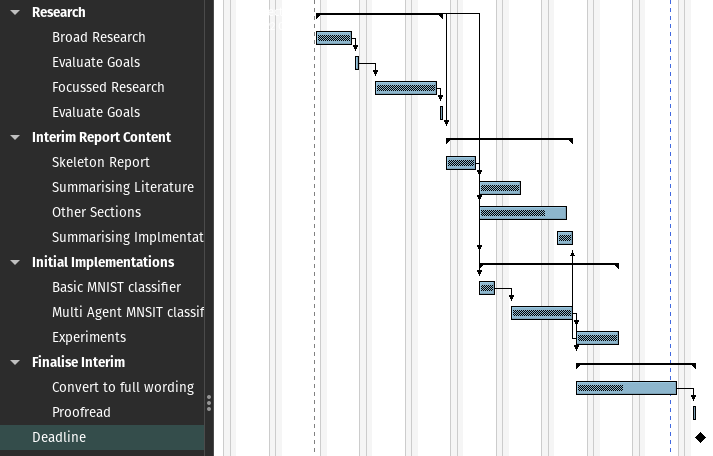
\includegraphics[width=\textwidth]{gantt_pre}
	\label{fig_g_pre}
	\caption{Gantt chart for pre-interim planning}
\end{figure}



\section{Remaining Work}
A second Gantt chart was created to plan the project after the interim stage. This chart includes plans for two problems, with a buffer in the form of the housekeeping phase in case of unforeseen delays. Only two problems were planned for however a third may be implemented if the project is ahead of schedule.

\begin{figure}[h]
	\centering
	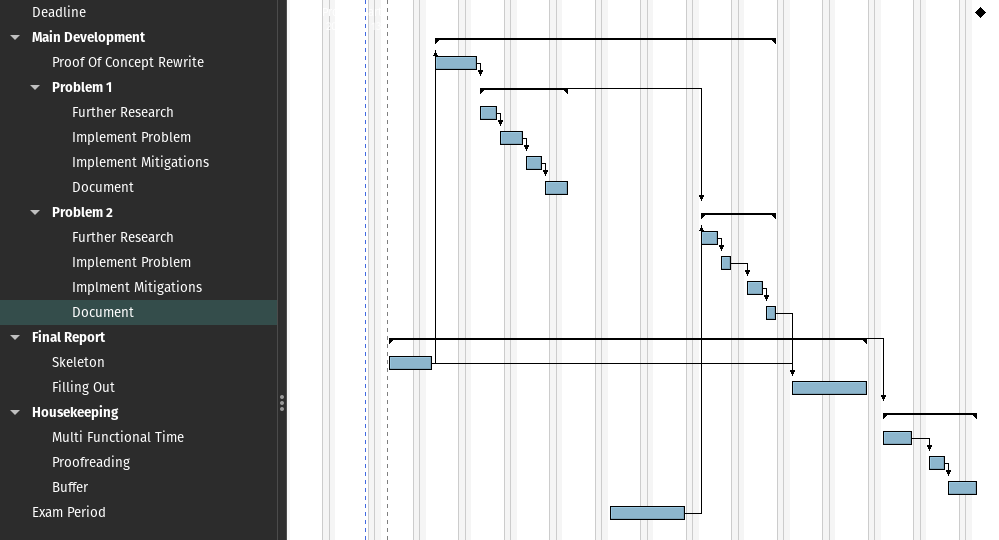
\includegraphics[width=\textwidth]{gantt_post}
	\label{fig_g_post}
	\caption{Gantt chart for post-interim planning}
\end{figure}


\section{Risk Assessment}
\subsection{Personal Issues}

\subsubsection{Description}
Personal issues which cause the author to be unable to do work, such as illness.

\subsubsection{Risk Calculations}
\emph{Severity (1-5):} 3 \\
\emph{Likelihood (1-5):} 3 \\
\emph{Overall Risk (1-25):} \textbf{9}

\subsubsection{Mitigation}
The codebase will be designed such that individual sections and modules have minimal dependencies on other sections. This means that, even if the author is unable to work for a period of time, some less critical sections can be omitted without significantly impacting the rest of the project.

\subsection{Hardware Failure}
\subsubsection{Description}
Failure on the authors local computer of any kind, such as a graphics card or storage breakage.

\subsubsection{Risk Calculations}
\emph{Severity (1-5):} 4 \\
\emph{Likelihood (1-5):} 2 \\
\emph{Overall Risk (1-25):} \textbf{8}

\subsubsection{Mitigation}
The project will be regularly backed up to GitHub. If a core component of the work computer breaks, the author has access to a personal laptop and the Zepler Labs. The deep learning environment along with dependencies is backed up to the authors Google Drive in the form of a docker image, so that switching to a new computer would be a smooth process.

\subsection{Algorithm Does Not Work Work}
\subsubsection{Description}
The SL algorithm does not function as well as expected. However, this is very unlikely as SL has been proven to work in numerous papers.

\subsubsection{Risk Calculations}
\emph{Severity (1-5):} 5 \\
\emph{Likelihood (1-5):} 1 \\
\emph{Overall Risk (1-25):} \textbf{5}

\subsubsection{Mitigation}
It may be possible to shift the project away from SL and onto distributed FL with leader election. FL is more commonly used and therefore has more literature, meaning that it is more likely to be an achievable goal to implement it.